\paragraph{Цель работы}
Научиться использовать библиотеку элементов графического интерфейса Qt.

\paragraph{Задание}
Калькулятор-конвертер для преобразования чисел из произвольных систем счисления в про-
извольные (можно ограничиться 16-ричной системой).

\lstinputlisting[language=C++]{../../src/QT/OSISP/number_caster/mainwindow.h}
\lstinputlisting[language=C++]{../../src/QT/OSISP/number_caster/mainwindow.cpp}

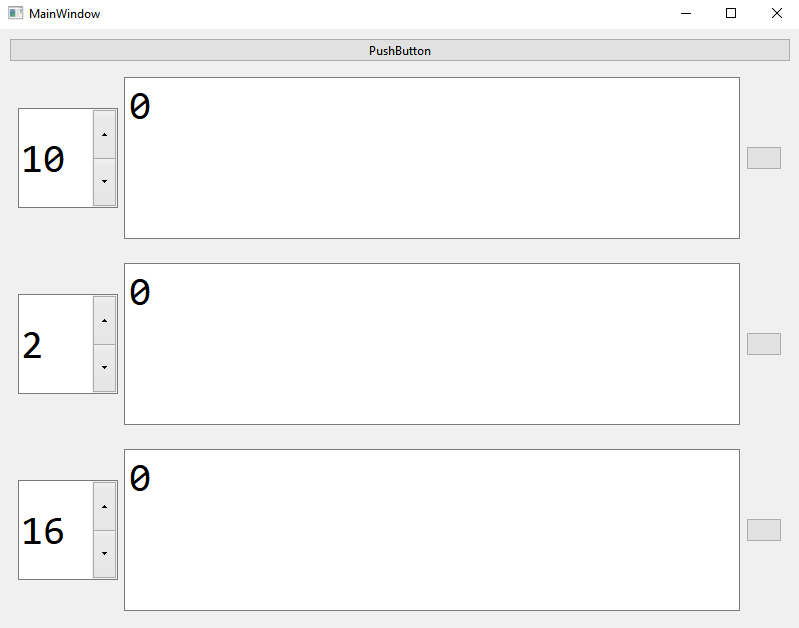
\includegraphics[width=0.6\textwidth]{scr1.PNG}

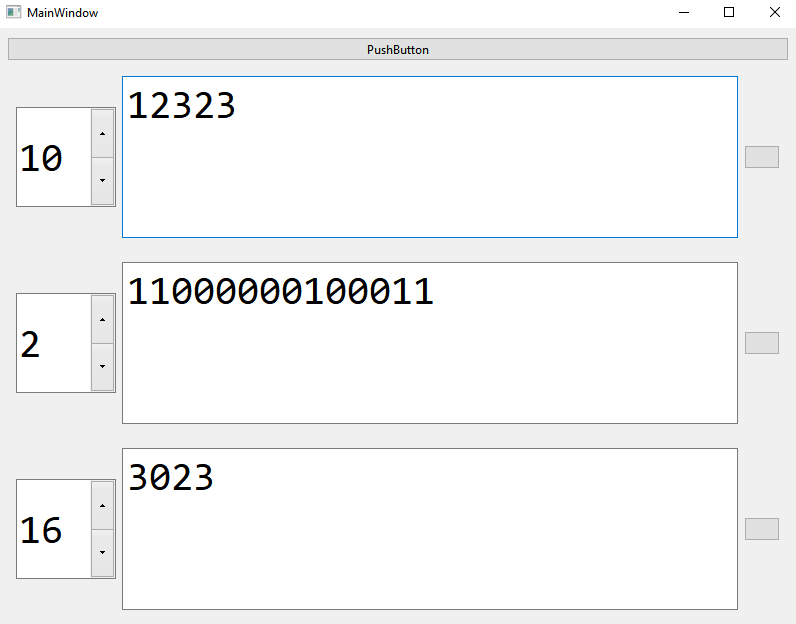
\includegraphics[width=0.6\textwidth]{scr2.PNG}

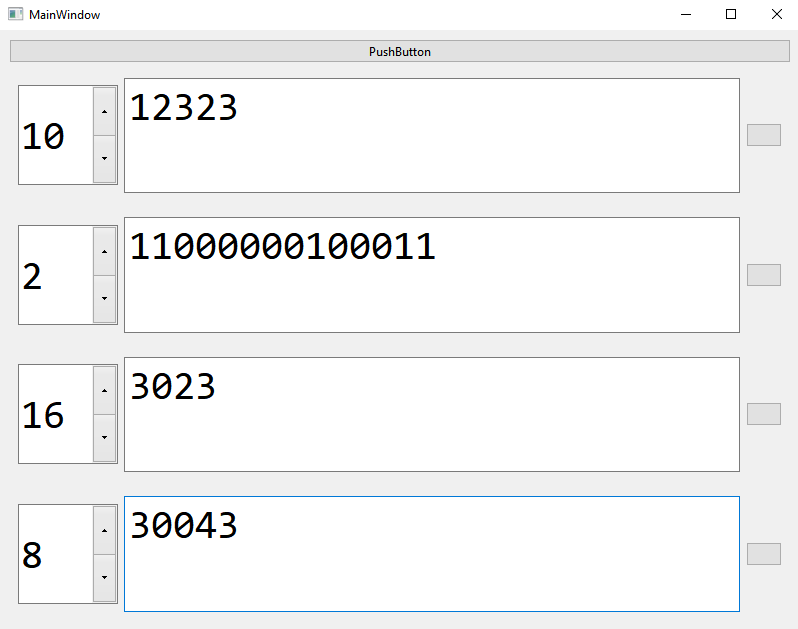
\includegraphics[width=0.6\textwidth]{scr3.PNG}


\includegraphics[width=0.6\textwidth]{scr4.PNG}